\documentclass{article}
\usepackage{amsmath}
\usepackage{amssymb}
\usepackage{tikz}
\usetikzlibrary{calc,patterns}
\usepackage[dvipsnames,svgnames]{xcolor}

\begin{document}

\section*{TUGAS MINGGU 1: SISTEM BILANGAN REAL}
\textbf{Tentukan Himpunan Penyelesaian (HP) untuk setiap pertidaksamaan berikut:}

\begin{enumerate}
    \item $2-3x \le 12$
    
    \textbf{Penyelesaian:}
    
    \begin{itemize}
    \item Langkah-langkah Penyelesaian
    
    \begin{align}
    2 - 3x &\leq 12 \quad \text{(Pertidaksamaan awal)} \\
    2 - 3x - 2 &\leq 12 - 2 \quad \text{(Kurangi 2 pada kedua ruas)} \\
    -3x &\leq 10 \quad \text{(Sederhanakan)} \\
    -3x \cdot \left(-\frac{1}{3}\right) &\geq 10 \cdot \left(-\frac{1}{3}\right) \quad \text{(Kali kedua ruas dengan $-\frac{1}{3}$)} \\
    x &\geq -\frac{10}{3} \quad \text{(Sederhanakan, tanda berubah)}
    \end{align}
    
    \item Gambar Garis Bilangan
    
    \begin{center}
    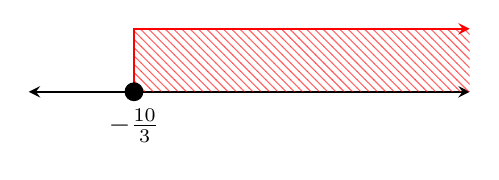
\begin{tikzpicture}[scale=0.8]
    
    % Gambar garis bilangan utama dengan panah di kedua ujung
    \draw[thick,stealth-stealth] (-5,0)--(2,0);
    
    % Gambar garis merah untuk himpunan penyelesaian (x ≥ -10/3)
    \draw[thick,-stealth,Red] (-3.33,0)--(-3.33,1)--(2,1);
    
    % Gambar arsiran untuk daerah penyelesaian
    \path[pattern=north west lines,opacity=.6,pattern color=Red] (-3.33,0)--(-3.33,1)--(2,1)--(2,0)--cycle;
    
    % Gambar lingkaran penuh di x = -10/3 (karena x ≥ -10/3)
    \filldraw[black,fill=black] (-3.33,0) node[below,yshift=-.1cm] {$-\frac{10}{3}$} circle (0.4em);
    
    \end{tikzpicture}
    \end{center}
    
    \item HP: $\left[-\frac{10}{3}, \infty\right)$
    \end{itemize}
    
    \item $3x-5 < 4x-6$
    
    \textbf{Penyelesaian:}
    
    \begin{itemize}
    \item Langkah-langkah Penyelesaian
    
    \begin{align}
    3x - 5 &< 4x - 6 \quad \text{(Pertidaksamaan awal)} \\
    3x - 5 - 4x &< 4x - 6 - 4x \quad \text{(Kurangi 4x pada kedua ruas)} \\
    3x - 4x - 5 &< 4x - 4x - 6 \quad \text{(Sederhanakan)} \\
    -x - 5 &< -6 \quad \text{(Sederhanakan)} \\
    -x - 5 + 5 &< -6 + 5 \quad \text{(Tambahkan 5 pada kedua ruas)} \\
    -x &< -1 \quad \text{(Sederhanakan)} \\
    -x \cdot (-1) &> -1 \cdot (-1) \quad \text{(Kali kedua ruas dengan -1)} \\
    x &> 1 \quad \text{(Sederhanakan, tanda berubah)}
    \end{align}
    
    \item Gambar Garis Bilangan
    
    \begin{center}
    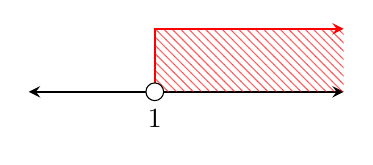
\begin{tikzpicture}[scale=0.8]
    
    % Gambar garis bilangan utama dengan panah di kedua ujung
    \draw[thick,stealth-stealth] (-1,0)--(4,0);
    
    % Gambar garis merah untuk himpunan penyelesaian (x > 1)
    \draw[thick,-stealth,Red] (1,0)--(1,1)--(4,1);
    
    % Gambar arsiran untuk daerah penyelesaian
    \path[pattern=north west lines,opacity=.6,pattern color=Red] (1,0)--(1,1)--(4,1)--(4,0)--cycle;
    
    % Gambar lingkaran kosong di x = 1 (karena x > 1, bukan x ≥ 1)
    \filldraw[black,fill=white] (1,0) node[below,yshift=-.1cm] {$1$} circle (0.4em);
    
    \end{tikzpicture}
    \end{center}
    
    \item HP: $(1, \infty)$
    \end{itemize}
    
    \item $-3 \le 1-6x < 4$
    
    \textbf{Penyelesaian:}
    
    \begin{itemize}
    \item Langkah-langkah Penyelesaian
    
    \begin{align}
    -3 &\leq 1-6x < 4 \quad \text{(Pertidaksamaan awal)} \\
    -3 - 1 &\leq 1-6x - 1 < 4 - 1 \quad \text{(Kurangi 1 pada semua bagian)} \\
    -4 &\leq -6x < 3 \quad \text{(Sederhanakan)} \\
    -4 \cdot \left(-\frac{1}{6}\right) &\geq -6x \cdot \left(-\frac{1}{6}\right) > 3 \cdot \left(-\frac{1}{6}\right) \quad \text{(Kali semua bagian dengan $-\frac{1}{6}$)} \\
    \frac{4}{6} &\geq x > -\frac{3}{6} \quad \text{(Sederhanakan, tanda berubah)} \\
    \frac{2}{3} &\geq x > -\frac{1}{2} \quad \text{(Sederhanakan pecahan)} \\
    -\frac{1}{2} &< x \leq \frac{2}{3} \quad \text{(Tulis ulang dalam bentuk standar)}
    \end{align}
    
    \item Gambar Garis Bilangan
    
    \begin{center}
    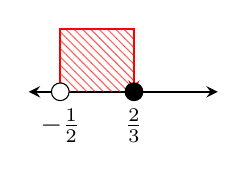
\begin{tikzpicture}[scale=0.8]
    
    % Gambar garis bilangan utama dengan panah di kedua ujung
    \draw[thick,stealth-stealth] (-1,0)--(2,0);
    
    % Gambar garis merah untuk himpunan penyelesaian (-1/2 < x ≤ 2/3)
    \draw[thick,-stealth,Red] (-0.5,0)--(-0.5,1)--(0.67,1)--(0.67,0);
    
    % Gambar arsiran untuk daerah penyelesaian
    \path[pattern=north west lines,opacity=.6,pattern color=Red] (-0.5,0)--(-0.5,1)--(0.67,1)--(0.67,0)--cycle;
    
    % Gambar lingkaran kosong di x = -1/2 (karena -1/2 < x) dan lingkaran penuh di x = 2/3 (karena x ≤ 2/3)
    \filldraw[black,fill=white] (-0.5,0) node[below,yshift=-.1cm] {$-\frac{1}{2}$} circle (0.4em);
    \filldraw[black,fill=black] (0.67,0) node[below,yshift=-.1cm] {$\frac{2}{3}$} circle (0.4em);
    
    \end{tikzpicture}
    \end{center}
    
    \item HP: $\left(-\frac{1}{2}, \frac{2}{3}\right]$
    \end{itemize}
    
    \item $2x^{2}-5x-3 < 0$
    
    \textbf{Penyelesaian:}
    
    \begin{itemize}
    \item Langkah-langkah Penyelesaian
    
    \begin{align}
    2x^2 - 5x - 3 &< 0 \quad \text{(Pertidaksamaan awal)} \\
    \text{Cari akar-akar persamaan } 2x^2 - 5x - 3 &= 0
    \end{align}
    
    \item Metode 1: Pemaktoran
    
    \begin{align}
    2x^2 - 5x - 3 &= 0 \\
    (2x + 1)(x - 3) &= 0 \quad \text{(Faktorkan)} \\
    2x + 1 &= 0 \quad \text{atau} \quad x - 3 = 0 \\
    2x &= -1 \quad \text{atau} \quad x = 3 \\
    x &= -\frac{1}{2} \quad \text{atau} \quad x = 3
    \end{align}
    
    \item Metode 2: Rumus ABC
    
    \begin{align}
    2x^2 - 5x - 3 &= 0 \\
    \text{Dengan } a = 2, b = -5, c = -3: & \\
    x_1,x_2 &= \frac{-b \pm \sqrt{b^2 - 4ac}}{2a} \\
    x_1,x_2 &= \frac{-(-5) \pm \sqrt{(-5)^2 - 4(2)(-3)}}{2(2)} \\
    x_1,x_2 &= \frac{5 \pm \sqrt{25 + 24}}{4} \\
    x_1,x_2 &= \frac{5 \pm \sqrt{49}}{4} \\
    x_1,x_2 &= \frac{5 \pm 7}{4} \\
    x_1 &= \frac{5 + 7}{4} = 3 \quad \text{atau} \quad x_2 = \frac{5 - 7}{4} = -\frac{1}{2}
    \end{align}
    
    \item Analisis Tanda
    
    Pilih nilai x yang representatif untuk setiap selang:
    
    \begin{align}
    \text{Selang } x < -\frac{1}{2}: \quad &\text{Pilih } x = -1 \\
    2x^2 - 5x - 3 &= 2(-1)^2 - 5(-1) - 3 = 2 + 5 - 3 = 4 > 0 \quad \text{(positif)} \\
    \text{Selang } -\frac{1}{2} < x < 3: \quad &\text{Pilih } x = 0 \\
    2x^2 - 5x - 3 &= 2(0)^2 - 5(0) - 3 = -3 < 0 \quad \text{(negatif)} \\
    \text{Selang } x > 3: \quad &\text{Pilih } x = 4 \\
    2x^2 - 5x - 3 &= 2(4)^2 - 5(4) - 3 = 32 - 20 - 3 = 9 > 0 \quad \text{(positif)}
    \end{align}
    
    \item Gambar Garis Bilangan dengan Analisis Tanda
    
    \begin{center}
    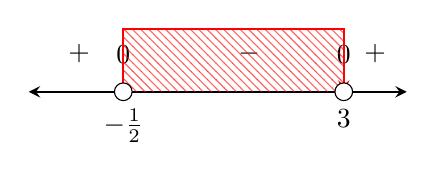
\begin{tikzpicture}[scale=0.8]
    
    % Gambar garis bilangan utama dengan panah di kedua ujung
    \draw[thick,stealth-stealth] (-2,0)--(4,0);
    
    % Gambar tanda pada setiap selang
    \node[above] at (-1.2,0.3) {$+$};
    \node[above] at (-0.5,0.3) {$0$};
    \node[above] at (1.5,0.3) {$-$};
    \node[above] at (3,0.3) {$0$};
    \node[above] at (3.5,0.3) {$+$};
    
    % Gambar garis merah untuk himpunan penyelesaian (-1/2 < x < 3)
    \draw[thick,-stealth,Red] (-0.5,0)--(-0.5,1)--(3,1)--(3,0);
    
    % Gambar arsiran untuk daerah penyelesaian
    \path[pattern=north west lines,opacity=.6,pattern color=Red] (-0.5,0)--(-0.5,1)--(3,1)--(3,0)--cycle;
    
    % Gambar lingkaran kosong di x = -1/2 dan x = 3 (karena -1/2 < x < 3)
    \filldraw[black,fill=white] (-0.5,0) node[below,yshift=-.1cm] {$-\frac{1}{2}$} circle (0.4em);
    \filldraw[black,fill=white] (3,0) node[below,yshift=-.1cm] {$3$} circle (0.4em);
    
    \end{tikzpicture}
    \end{center}
    
    \item HP: $\left(-\frac{1}{2}, 3\right)$
    \end{itemize}
    
    \item $x^{2}-5x-6 \le 0$
    
    \textbf{Penyelesaian:}
    
    \begin{itemize}
    \item Langkah-langkah Penyelesaian
    
    \begin{align}
    x^2 - 5x - 6 &\leq 0 \quad \text{(Pertidaksamaan awal)} \\
    \text{Cari akar-akar persamaan } x^2 - 5x - 6 &= 0
    \end{align}
    
    \item Metode 1: Pemaktoran
    
    \begin{align}
    x^2 - 5x - 6 &= 0 \\
    (x - 6)(x + 1) &= 0 \quad \text{(Faktorkan)} \\
    x - 6 &= 0 \quad \text{atau} \quad x + 1 = 0 \\
    x &= 6 \quad \text{atau} \quad x = -1
    \end{align}
    
    \item Metode 2: Rumus ABC
    
    \begin{align}
    x^2 - 5x - 6 &= 0 \\
    \text{Dengan } a = 1, b = -5, c = -6: & \\
    x_1,x_2 &= \frac{-b \pm \sqrt{b^2 - 4ac}}{2a} \\
    x_1,x_2 &= \frac{-(-5) \pm \sqrt{(-5)^2 - 4(1)(-6)}}{2(1)} \\
    x_1,x_2 &= \frac{5 \pm \sqrt{25 + 24}}{2} \\
    x_1,x_2 &= \frac{5 \pm \sqrt{49}}{2} \\
    x_1,x_2 &= \frac{5 \pm 7}{2} \\
    x_1 &= \frac{5 + 7}{2} = 6 \quad \text{atau} \quad x_2 = \frac{5 - 7}{2} = -1
    \end{align}
    
    \item Analisis Tanda
    
    Pilih nilai x yang representatif untuk setiap selang:
    
    \begin{align}
    \text{Selang } x < -1: \quad &\text{Pilih } x = -2 \\
    x^2 - 5x - 6 &= (-2)^2 - 5(-2) - 6 = 4 + 10 - 6 = 8 > 0 \quad \text{(positif)} \\
    \text{Selang } -1 < x < 6: \quad &\text{Pilih } x = 0 \\
    x^2 - 5x - 6 &= (0)^2 - 5(0) - 6 = -6 < 0 \quad \text{(negatif)} \\
    \text{Selang } x > 6: \quad &\text{Pilih } x = 7 \\
    x^2 - 5x - 6 &= (7)^2 - 5(7) - 6 = 49 - 35 - 6 = 8 > 0 \quad \text{(positif)} \\
    \text{Titik Potong }: \quad & x = -1 \\
    x^2 - 5x - 6 &= (-1)^2 - 5(-1) - 6 = 1 + 5 - 6 = 0 \quad \text{(nol)} \\
    \text{Titik Potong }: \quad & x = 6 \\
    x^2 - 5x - 6 &= (6)^2 - 5(6) - 6 = 36 - 30 - 6 = 0 \quad \text{(nol)}
    \end{align}
    
    \item Gambar Garis Bilangan dengan Analisis Tanda
    
    \begin{center}
    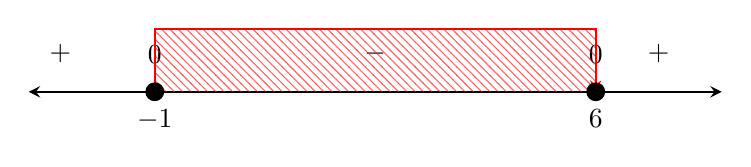
\begin{tikzpicture}[scale=0.8]
    
    % Gambar garis bilangan utama dengan panah di kedua ujung
    \draw[thick,stealth-stealth] (-3,0)--(8,0);
    
    % Gambar tanda pada setiap selang
    \node[above] at (-2.5,0.3) {$+$};
    \node[above] at (-1,0.3) {$0$};
    \node[above] at (2.5,0.3) {$-$};
    \node[above] at (6,0.3) {$0$};
    \node[above] at (7,0.3) {$+$};
    
    % Gambar garis merah untuk himpunan penyelesaian (-1 ≤ x ≤ 6)
    \draw[thick,-stealth,Red] (-1,0)--(-1,1)--(6,1)--(6,0);
    
    % Gambar arsiran untuk daerah penyelesaian
    \path[pattern=north west lines,opacity=.6,pattern color=Red] (-1,0)--(-1,1)--(6,1)--(6,0)--cycle;
    
    % Gambar lingkaran penuh di x = -1 dan x = 6 (karena -1 ≤ x ≤ 6)
    \filldraw[black,fill=black] (-1,0) node[below,yshift=-.1cm] {$-1$} circle (0.4em);
    \filldraw[black,fill=black] (6,0) node[below,yshift=-.1cm] {$6$} circle (0.4em);
    
    \end{tikzpicture}
    \end{center}
    
    \item HP: $[-1, 6]$
    \end{itemize}
    
    \item $\displaystyle \frac{1}{x+1} < \frac{2}{3x-1}$
    
    \textbf{Penyelesaian:}
    
    \begin{itemize}
    \item Langkah-langkah Penyelesaian
    
    \begin{align}
    \frac{1}{x+1} &< \frac{2}{3x-1} \quad \text{(Pertidaksamaan awal)} \\
    \frac{1}{x+1} - \frac{2}{3x-1} &< \frac{2}{3x-1} - \frac{2}{3x-1} \quad \text{(Kurangi $\frac{2}{3x-1}$ pada semua ruas)} \\
    \frac{1}{x+1} - \frac{2}{3x-1} &< 0 \quad \text{(Sederhanakan)} \\
    \frac{1(3x-1) - 2(x+1)}{(x+1)(3x-1)} &< 0 \quad \text{(Samakan penyebut)} \\
    \frac{3x-1-2x-2}{(x+1)(3x-1)} &< 0 \quad \text{(Sederhanakan pembilang)} \\
    \frac{x-3}{(x+1)(3x-1)} &< 0 \quad \text{(Sederhanakan)}
    \end{align}
    
    \item Tentukan Titik Kritis
    
    Pembuat nol pembilang dan penyebut:
    \begin{align}
    x-3 &= 0 \Rightarrow x = 3 \quad \text{(Pembuat nol pembilang)} \\
    x+1 &= 0 \Rightarrow x = -1 \quad \text{(Pembuat nol penyebut)} \\
    3x-1 &= 0 \Rightarrow x = \frac{1}{3} \quad \text{(Pembuat nol penyebut)}
    \end{align}
    
    \item Analisis Tanda
    
    Pilih nilai x yang representatif untuk setiap selang:
    
    \begin{align}
    \text{Selang } x < -1: \quad &\text{Pilih } x = -2 \\
    \frac{x-3}{(x+1)(3x-1)} &= \frac{-2-3}{(-2+1)(3(-2)-1)} = \frac{-5}{(-1)(-7)} = \frac{-5}{7} < 0 \quad \text{(negatif)} \\
    \text{Selang } -1 < x < \frac{1}{3}: \quad &\text{Pilih } x = 0 \\
    \frac{x-3}{(x+1)(3x-1)} &= \frac{0-3}{(0+1)(3(0)-1)} = \frac{-3}{(1)(-1)} = \frac{-3}{-1} = 3 > 0 \quad \text{(positif)} \\
    \text{Selang } \frac{1}{3} < x < 3: \quad &\text{Pilih } x = 1 \\
    \frac{x-3}{(x+1)(3x-1)} &= \frac{1-3}{(1+1)(3(1)-1)} = \frac{-2}{(2)(2)} = \frac{-2}{4} = -\frac{1}{2} < 0 \quad \text{(negatif)} \\
    \text{Selang } x > 3: \quad &\text{Pilih } x = 4 \\
    \frac{x-3}{(x+1)(3x-1)} &= \frac{4-3}{(4+1)(3(4)-1)} = \frac{1}{(5)(11)} = \frac{1}{55} > 0 \quad \text{(positif)}
    \end{align}
    
    \item Gambar Garis Bilangan dengan Analisis Tanda
    
    \begin{center}
    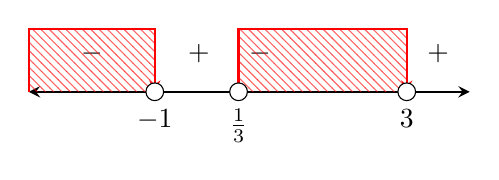
\begin{tikzpicture}[scale=0.8]
    
    % Gambar garis bilangan utama dengan panah di kedua ujung
    \draw[thick,stealth-stealth] (-3,0)--(4,0);
    
    % Gambar tanda pada setiap selang
    \node[above] at (-2,0.3) {$-$};
    \node[above] at (-0.3,0.3) {$+$};
    \node[above] at (0.67,0.3) {$-$};
    \node[above] at (3.5,0.3) {$+$};
    
    % Gambar garis merah untuk himpunan penyelesaian (x < -1 atau 1/3 < x < 3)
    \draw[thick,-stealth,Red] (-3,0)--(-3,1)--(-1,1)--(-1,0);
    \draw[thick,-stealth,Red] (0.33,0)--(0.33,1)--(3,1)--(3,0);
    
    % Gambar arsiran untuk daerah penyelesaian
    \path[pattern=north west lines,opacity=.6,pattern color=Red] (-3,0)--(-3,1)--(-1,1)--(-1,0)--cycle;
    \path[pattern=north west lines,opacity=.6,pattern color=Red] (0.33,0)--(0.33,1)--(3,1)--(3,0)--cycle;
    
    % Gambar lingkaran kosong di titik kritis (karena tidak termasuk)
    \filldraw[black,fill=white] (-1,0) node[below,yshift=-.1cm] {$-1$} circle (0.4em);
    \filldraw[black,fill=white] (0.33,0) node[below,yshift=-.1cm] {$\frac{1}{3}$} circle (0.4em);
    \filldraw[black,fill=white] (3,0) node[below,yshift=-.1cm] {$3$} circle (0.4em);
    
    \end{tikzpicture}
    \end{center}
    
    \item HP: $(-\infty, -1) \cup \left(\frac{1}{3}, 3\right)$
    \end{itemize}
    
    \item $\displaystyle \frac{x+2}{x+4} < \frac{x-1}{x-2}$
    
    \textbf{Penyelesaian:}
    
    \begin{itemize}
    \item Langkah-langkah Penyelesaian
    
    \begin{align}
    \frac{x+2}{x+4} &< \frac{x-1}{x-2} \quad \text{(Pertidaksamaan awal)} \\
    \frac{x+2}{x+4} - \frac{x-1}{x-2} &< \frac{x-1}{x-2} - \frac{x-1}{x-2} \quad \text{(Kurangi $\frac{x-1}{x-2}$ pada semua ruas)} \\
    \frac{x+2}{x+4} - \frac{x-1}{x-2} &< 0 \quad \text{(Sederhanakan)} \\
    \frac{(x+2)(x-2) - (x-1)(x+4)}{(x+4)(x-2)} &< 0 \quad \text{(Samakan penyebut)} \\
    \frac{(x+2)(x-2) - (x-1)(x+4)}{(x+4)(x-2)} &< 0 \quad \text{(Sederhanakan pembilang)} \\
    \frac{x^2-4-(x^2+3x-4)}{(x+4)(x-2)} &< 0 \quad \text{(Ekspansi)} \\
    \frac{x^2-4-x^2-3x+4}{(x+4)(x-2)} &< 0 \quad \text{(Sederhanakan)} \\
    \frac{-3x}{(x+4)(x-2)} &< 0 \quad \text{(Sederhanakan)}
    \end{align}
    
    \item Tentukan Titik Kritis
    
    Pembuat nol pembilang dan penyebut:
    \begin{align}
    -3x &= 0 \Rightarrow x = 0 \quad \text{(Pembuat nol pembilang)} \\
    x+4 &= 0 \Rightarrow x = -4 \quad \text{(Pembuat nol penyebut)} \\
    x-2 &= 0 \Rightarrow x = 2 \quad \text{(Pembuat nol penyebut)}
    \end{align}
    
    \item Analisis Tanda
    
    Pilih nilai x yang representatif untuk setiap selang:
    
    \begin{align}
    \text{Selang } x < -4: \quad &\text{Pilih } x = -5 \\
    \frac{-3x}{(x+4)(x-2)} &= \frac{-3(-5)}{(-5+4)(-5-2)} = \frac{15}{(-1)(-7)} = \frac{15}{7} > 0 \quad \text{(positif)} \\
    \text{Selang } -4 < x < 0: \quad &\text{Pilih } x = -1 \\
    \frac{-3x}{(x+4)(x-2)} &= \frac{-3(-1)}{(-1+4)(-1-2)} = \frac{3}{(3)(-3)} = \frac{3}{-9} = -\frac{1}{3} < 0 \quad \text{(negatif)} \\
    \text{Selang } 0 < x < 2: \quad &\text{Pilih } x = 1 \\
    \frac{-3x}{(x+4)(x-2)} &= \frac{-3(1)}{(1+4)(1-2)} = \frac{-3}{(5)(-1)} = \frac{-3}{-5} = \frac{3}{5} > 0 \quad \text{(positif)} \\
    \text{Selang } x > 2: \quad &\text{Pilih } x = 3 \\
    \frac{-3x}{(x+4)(x-2)} &= \frac{-3(3)}{(3+4)(3-2)} = \frac{-9}{(7)(1)} = \frac{-9}{7} < 0 \quad \text{(negatif)} \\
    \text{Titik Kritis }: \quad & x = -4, x = 0, x = 2 \quad \text{(Tidak termasuk karena penyebut nol atau pembilang nol)}
    \end{align}
    
    \item Gambar Garis Bilangan dengan Analisis Tanda
    
    \begin{center}
    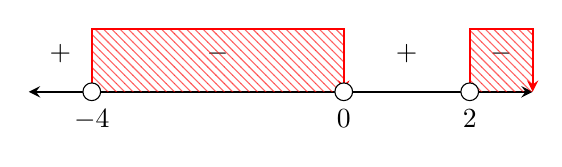
\begin{tikzpicture}[scale=0.8]
    
    % Gambar garis bilangan utama dengan panah di kedua ujung
    \draw[thick,stealth-stealth] (-5,0)--(3,0);
    
    % Gambar tanda pada setiap selang
    \node[above] at (-4.5,0.3) {$+$};
    \node[above] at (-2,0.3) {$-$};
    \node[above] at (1,0.3) {$+$};
    \node[above] at (2.5,0.3) {$-$};
    
    % Gambar garis merah untuk himpunan penyelesaian (-4 < x < 0 atau x > 2)
    \draw[thick,-stealth,Red] (-4,0)--(-4,1)--(0,1)--(0,0);
    \draw[thick,-stealth,Red] (2,0)--(2,1)--(3,1)--(3,0);
    
    % Gambar arsiran untuk daerah penyelesaian
    \path[pattern=north west lines,opacity=.6,pattern color=Red] (-4,0)--(-4,1)--(0,1)--(0,0)--cycle;
    \path[pattern=north west lines,opacity=.6,pattern color=Red] (2,0)--(2,1)--(3,1)--(3,0)--cycle;
    
    % Gambar lingkaran kosong di titik kritis (karena tidak termasuk)
    \filldraw[black,fill=white] (-4,0) node[below,yshift=-.1cm] {$-4$} circle (0.4em);
    \filldraw[black,fill=white] (0,0) node[below,yshift=-.1cm] {$0$} circle (0.4em);
    \filldraw[black,fill=white] (2,0) node[below,yshift=-.1cm] {$2$} circle (0.4em);
    
    \end{tikzpicture}
    \end{center}
    
    \item HP: $(-4, 0) \cup (2, \infty)$
    \end{itemize}
\end{enumerate}

\end{document}